\documentclass[a4paper,10pt]{article}
\usepackage[utf8]{inputenc}

% ----  Useful packages % ---- 
\usepackage{amsmath}
\usepackage{graphicx}
\usepackage{amsfonts}
\usepackage{amsthm}
\usepackage{amssymb}
\usepackage{makecell}
\usepackage{array}
\usepackage{booktabs}
\usepackage{multirow}
\usepackage{subfigure}
% ----  Useful packages % ---- 

\usepackage{wrapfig}
\usepackage{caption}
\usepackage{subcaption}
\usepackage{hyperref}
\hypersetup{
    colorlinks,
    citecolor=black,
    filecolor=black,
    linkcolor=black,
    urlcolor=black
}

\graphicspath{ {./images/} }

% ---- Set page size and margins replace ------
\usepackage[letterpaper,top=2cm,bottom=2cm,left=3cm,right=3cm,marginparwidth=1.75cm]{geometry}
% ---- Set page size and margins replace ------

% ------- NOTA ------
\theoremstyle{remark}
\newtheorem{note}{Note}[subsubsection]
% ------- NOTA ------

% ------- OSSERVAZIONE ------
\theoremstyle{definition}
\newtheorem{observation}{Observation}[subsection]
% ------- OSSERVAZIONE ------

% ------- DEFINIZIONE ------
\theoremstyle{plain}
\newtheorem{definition}{Definition}[subsection]
% ------- DEFINIZIONE ------

% ------- ESEMPIO ------
\theoremstyle{definition}
\newtheorem{example}{Example}[subsection]
% ------- ESEMPIO ------

% ------- DIMOSTRAZIONE ------
\theoremstyle{definition}
\newtheorem{demostration}{Dimostrazione}[subsection]
% ------- DIMOSTRAZIONE ------

% ------- TEOREMA ------
\theoremstyle{definition}
\newtheorem{theorem}{Theorem}[subsection]
% ------- TEOREMA ------

% ------- COROLLARIO ------
\theoremstyle{plain}
\newtheorem{corollaries}{Corollario}[theorem]
% ------- COROLLARIO ------

% ------- PROPOSIZIONE ------
\theoremstyle{plain}
\newtheorem{proposition}{Proposizione}[subsection]
% ------- PROPOSIZIONE ------

% ---- Footer and header ---- 
\usepackage{fancyhdr}
\pagestyle{fancy}
\fancyhf{}
\fancyhead[LE,RO]{A.A 2024-2025}
\fancyhead[RE,LO]{Machine Learning for Data Science}
\fancyfoot[RE,LO]{\rightmark}
\fancyfoot[LE,RO]{\thepage}

\renewcommand{\headrulewidth}{.5pt}
\renewcommand{\footrulewidth}{.5pt}
% ---- Footer and header ---- 

% ----  Language setting ---- 
\usepackage[italian, english]{babel}
% ----  Language setting ---- 

\usepackage{listings}
\usepackage{color}

\definecolor{dkgreen}{rgb}{0,0.6,0}
\definecolor{gray}{rgb}{0.5,0.5,0.5}
\definecolor{mauve}{rgb}{0.58,0,0.82}

\lstset{frame=tb,
  language=C,
  aboveskip=3mm,
  belowskip=3mm,
  showstringspaces=false,
  columns=flexible,
  basicstyle={\small\ttfamily},
  numbers=none,
  numberstyle=\tiny\color{gray},
  keywordstyle=\color{blue},
  commentstyle=\color{dkgreen},
  stringstyle=\color{mauve},
  breaklines=true,
  breakatwhitespace=true,
  tabsize=3
}

\title{\textbf{Machine learning for data science}}
\author{Autor: Ghirardini Filippo}
\date{Winter Semester 2024-2025}

\begin{document}
\begin{titlepage} %crea l'enviroment
	\begin{figure}[t] %inserisce le figure
		\centering
\includegraphics[width=0.98\textwidth]{marchio_unipi_pant541.png}
	\end{figure}
	\vspace{20mm}
	
	\begin{Large}
		\begin{center}
			\textbf{Dipartimento di Informatica\\ Corso di Laurea Triennale in Informatica\\}
			\vspace{20mm}
			{\LARGE{Corso a Libera Scelta - 6 CFU}}\\
			\vspace{10mm}
			{\huge{\bf Computer Graphics}}\\
		\end{center}
	\end{Large}
	
	
	\vspace{36mm}
	%minipage divide la pagina in due sezioni settabili
	\begin{minipage}[t]{0.47\textwidth}
		{\large{\bf Professore:}\\ \large{Prof. }}
	\end{minipage}
	\hfill
	\begin{minipage}[t]{0.47\textwidth}\raggedleft
		{\large{\bf Autore:}\\ \large{Filippo Ghirardini}}
	\end{minipage}
	
	\vspace{25mm}
	
	\hrulefill
	
	\vspace{5mm}
	
	\centering{\large{\bf Anno Accademico 2023/2024 }}
	
\end{titlepage}

\tableofcontents
\newpage
\maketitle
\begin{center}
    \vspace{-20pt}
    \rule{11cm}{.1pt} 
\end{center}
\newpage
\section{Punto materiale}
Oggetto caratterizzato da una massa [kg] e da un vettore posizione [m] nello spazio 3D.
Dimensioni trascurabili, forma irrilevante rispetto ai fenomeni di interesse.
Vettore posizione come funzione del tempo t[s].
\begin{example}
    Una molecola di ossigeno se sono interessato all'aereodinamica di una vettua. 
    Un satellite attorno alla terra se ignoro le forze di marea.
\end{example}
\hspace{-15pt}\textbf{Un vettore posizione} è una funzione del tempo $t[s]$.
$$\vec{r(t)} = (x(t), y(t), z(t)) = x(t)\hat{x} + y(t)\hat{z} + z(t)\hat{z}$$
\begin{observation}
    I versori cartesiani sono costanti
\end{observation}

\begin{definition}[Legge oraria]
    Si definisce come legge oraria la funzione $t \mapsto \vec{r}(t)$.
\end{definition}

\begin{definition}[Traiettoria]
    Il luogo geometrico di punti visitati dal punto materiale.
    $$\{\vec{r}(t)\:\: per \: t \in \mathbb{R}\}$$
\end{definition}

\begin{example}
    $\vec{r}(t) = (v_0t, y_0, 0)$ e $v_0 = 3m/s, y_o = 5m$ 
    \begin{figure}[h!]
        \centering
        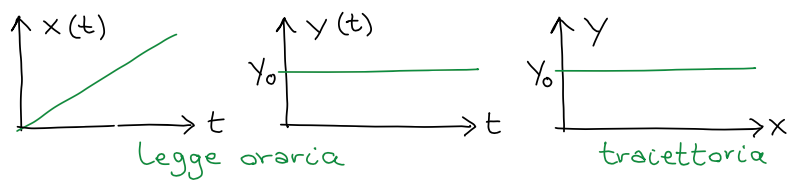
\includegraphics[width=0.8\textwidth]{images/ess-traiettoria.png}
    \end{figure}
\end{example}

\begin{definition}
    La \textbf{velocità istantanea} è la derivata della posizione rispetto al tempo.
    $$v = \lim_{\Delta t \to 0}\frac{\Delta s}{\Delta t} = \frac{ds}{dt}$$
\end{definition}

\begin{definition}
    La \textbf{velocità media} è definita come il rapporto tra lo spostamento e l'intervallo di tempo necessario per effettuarlo.
    $$v_m = \frac{\Delta s}{\Delta t}$$
\end{definition}
\hspace{-15pt}In parole povere è una grandezza che ci dice con quale rapidità cambia la posizione di un punto rispetto al tempo nell'instante $t$.
\subsection*{Vettore velocità}
Derivata rispetto al tempo del vettore posizione e si indica come 
$\frac{d\vec{r}(t)}{dt}\text{ oppure }\dot{\vec{r}}(t)[m/s]$
\begin{equation}
    \begin{split}
    \dot{\vec{r}}(t) & = (\dot{x}(t), \dot{y}(t), \dot{z}(t)) \\
     & = \frac{d}{dt}[x(t)\hat{x} + y(t)\hat{y} + z(t)\hat{z}] \\
     & = \dot{x}(t)\hat{x} + \dot{y}(t)\hat{y} + \dot{z}(t)\hat{z}
    \end{split}
\end{equation}
Per ricavare la forma esplicita uso le proprietà delle derivate (\textbf{linearità}, \textbf{Leibnitz})
\begin{example}
    $\vec{r}(t) = (v_0t, y_0, 0) = v_0t\hat{x} + y_0\hat{y}$ \:\:\:abbiamo che \:\:\:
    $\dot{\vec{r}}(t) = (v_0, 0, 0) = v_0 \hat{x}$
\end{example}
\hspace{-15pt}Velocità e spazio percorso ("integrale di linea").\\
\begin{wrapfigure}[3]{l}{5cm}
    \centering
    \includegraphics[width=5cm]{images/vettore-velocità.png}
\end{wrapfigure}
\begin{align*}
    L & = ||\vec{r}(t_1) - \vec{r}(t_0)|| + ||\vec{r}(t_2) - \vec{r}(t_1)|| + ||\vec{r}(t_3) - \vec{r}(t_2)|| + \dots \\
    & = \sum_i ||\vec{r}(t_{i+1} - \vec{r}(t_i)|| \:\: per\:\: |t_{i+1} - t_i| \text{"piccolo"} \\
    & = \sum_i ||\frac{\vec{r}(t_{i+1}) - \vec{r}(t_i)}{t_{i+1} - t_i}|| (t_{i+1} - t_i) = \int_{t_{in}}^{t_{f_{in}}}||\dot{\vec{r}}(t)||\\
\end{align*}
\begin{example}
    $\vec{r}(t) = (v_0t, y_0)\:\:\: \dot{\vec{r}}(t) = (v_0, 0)$\hspace{15pt}
    $||\dot{\vec{r}}(t)|| = \sqrt{v_0^2 + 0^2} = |v_0|$ \:\:\: $L = |v_0| \cdot (t_{f_{in}} - t_{in})$\\
    Il vettore è costante quindi facendo la derivata torna zero. Con la velocità si calcolo lo spazio percorso ("integrale di linea").
    La differenza fra le posizioni e la differenza dei tempi è il rapporto incrementale in caso gli intervalli siano sufficentemente
    piccoli, da qui si ottiene l'integrale.
\end{example}

\subsection{Vettore accelerazione}
Derivata rispetto al tempo del vettore velocità e si indica con $\frac{d^2\vec{r}(t)}{dt} \text{ oppure } \ddot{\vec{r}}(t) [m/s^2]$
\begin{equation}
    \ddot{\vec{r}}(t) = (\ddot{x}(t), \ddot{y}(t), \ddot{z}(t))\:\: = \:\: \ddot{x}(t)\hat{x} + \ddot{y}(t)\hat{y} + \ddot{z}(t)\hat{z}
\end{equation}
\begin{example}
    $\vec{r}(t)= (\frac{1}{2}a_0t^2, v_0t, 0)$ \hspace{10pt} $\dot{\vec{r}}(t) = (a_0t, v_0, 0)$ \hspace{10pt} $\dot{\vec{r}}(t) = (a_0, 0, 0)$
\end{example}
\hspace{-15pt}Serve perché l'equazione "del moto" di Newton che determinata la legge oraria è formulata in termini di accelerazione.

\subsection{Vettore quantità di moto}
Il prodotto di massa [kg] e velocità [m/s]
$$\vec{p}(t) = m \cdot \dot{\vec{r}}(t) = (m\dot{x}(t), m\dot{y}(t), m\dot{x}(t)) = m\dot{\vec{x}}(t)x + m\dot{\vec{y}}(t)y + m \dot{\vec{z}}(t)z$$
\begin{example}
    Prendiamo un punto di massa 2kg e velocità 3m/s lungo $\hat{x}$.\\
    $p_x(t) = 2 \cdot 3 kg\cdot m/s = 6 kg \cdot m/s$ \hspace{15pt} $p_y(t) = p_z(t) = 0$.
\end{example}
\hspace{-15pt}Serve per generalizzare l'equazione di Newton e per trattare sistemi di piu punti materiali.

\subsection{Vettore momento angolare rispetto a un polo P}
$$\vec{L}_p(t) = m(\vec{r}(t) - \vec{r}_p) \times \dot{\vec{r}}(t)$$
Dove $\vec{r}_p$ è il vettore posizione di p, mentre $\dot{\vec{r}}(t)$ è il prodotto vettoriale.
\begin{example}
    $\vec{r}_p = (l_0, 0, 0)$ \hspace{15pt} $\vec{r}(t) = (v_0t, y_0, 0)$\\
    $\vec{L}_p = m[(v_0t - l_0)\hat{x} + y_0\hat{y}] \times (v_0\hat{x}) \:\: = \:\: m(v_0t - l_0)v_0 \hat{x} \times \hat{x} + my_0v_0\hat{y}\times \hat{x} 
    \:\: = \:\: my_0v_0(-\hat{z}) = (0,0, -my_0v_0)$\\
    Ricorda che $\hat{x} \times \hat{x} = 0$ e $\hat{y} \times \hat{x} = -\hat{z}$
\end{example}
\hspace{-15pt}Il momento angolare dice quanta inerzia ha un oggetto in una rotazione (descrizione sommaria).\\
Il polo P è parte della definizione. È una scelta! Il risultato dipende dal polo.
Serve per formulare l'equazione del moto di sistemi di punti materiali e corpi rigidi.

\subsection{Coordinate polari}
Un metodo per rapprensentare delle cordinate x, y andando a misurare prima la distanza dall'origine e poi si va a vedere
quanto vale l'angolo fra questo segmento dall'asse x, utilizzando seno e coseno.
\begin{wrapfigure}[7]{l}{2cm}
    \centering
    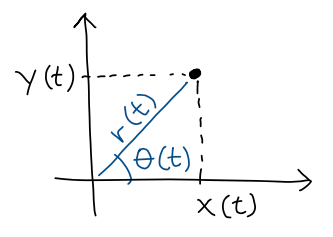
\includegraphics[width=5.5cm]{images/coordinate-polari.png}
\end{wrapfigure}
\begin{align*}
    \begin{cases}
        x(t) = r(t) \cdot \cos(\Theta(t))\\
        y(t) = r(t) \cdot \sin(\Theta(t)) 
    \end{cases}
\end{align*}
\begin{align*}
    \begin{cases}
        r(t) = \sqrt{x(t)^2 + y(t)^2} \geq 0\\
        tg(\Theta(t)) = y(t) / x(t) 
    \end{cases}
\end{align*}
\\
\begin{example} Esempi di rappresentazione di coordinate in coordinate polari.\\
    $x = 0, y = l_0 > 0 \:\: \Rightarrow \:\: r = l_0, \Theta = \pi/2$\\
    $x = 0, y = -l_0 < 0 \:\: \Rightarrow \:\: r = l_0, \Theta = -\pi/2$\\
    $x = l_0, y = l_0 > 0 \:\: \Rightarrow \:\: r = \sqrt{2}l_0, \Theta = \pi/4$\\
\end{example}

\subsection{Versori polari (2D)}
Definisco un versore $\hat{r}(t)$ che punta verso il punto materiale e un versore $\hat{\Theta}(t)$ ortogonale.
Si esprime facilmente in coordinte polari.
$$\vec{r}(t) = (x(t), y(t)) = (r(t)\cos \Theta(t), r(t)\sin\Theta(t)) \:\: = \:\: r(t)(\cos\Theta(t)\hat{x} + \sin\Theta(t)\hat{y})$$
Ma $||\vec{r}(t)|| = |r(t)| = r(t)$ allora definisco $\hat{r}(t) = \vec{r}(t)/ ||\vec{r}(t)|| = \cos \Theta(t)\hat{x} + \sin\Theta(t)\hat{y}$\\\\
Trovo facilmente che un versore ortogonale è:
$$\hat{\Theta(t)} = -\sin\Theta(t)\hat{x} + \cos\Theta(t)\hat{y} \:\:\:\text{infatti} \:\:\: \hat{r}\cdot \hat{\Theta} = c \cdot (-s) + s \cdot c = 0$$
\begin{wrapfigure}[7]{r}{6cm}
    \centering
    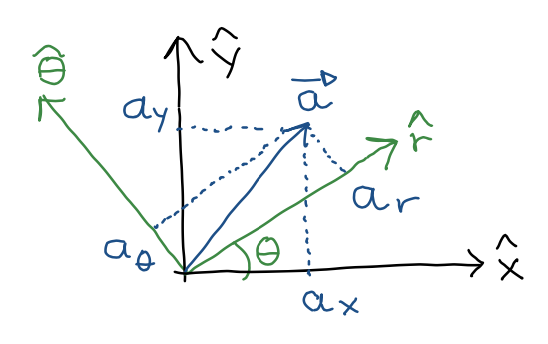
\includegraphics[width=5.5cm]{images/trasformazioni-inverse.png}
\end{wrapfigure}
\begin{note}
    Non c'è legame fra $\Theta$ e $\hat{\Theta}$ è solo una convenzione.
\end{note}
\hspace{-15pt}Le trasformazioni inverse invece si fanno come segue (verifico per sostituzione):
$$\hat{y} = \cos\Theta(t)\hat{r} - \sin\Theta(t)\hat{\Theta} \hspace{20pt} \hat{y} = \sin\Theta(t)\hat{r} + \cos\Theta(t)\hat{\Theta}$$
Possono quindi scrivere ogni vettore nella forma $\vec{a} = a_r\hat{r} + a_{\Theta}\hat{\Theta}$ con le componenti polari $a_r, a_{\Theta}$.
Per evitare ambiguità non scriviamo $(a_r, a_{\Theta})$ e riserviamo la notazione alle componenti cartesiane.\\\\
A differenza dei versori cartesiani quelli polari dipendono dal tempo per costruzioni.
$$\dot{\hat{r}}(t) = \frac{d}{dt}[\cos\Theta(t) \hat{x} + \sin\Theta(t)\hat{y}] \:\: = \:\: -\sin\Theta(t) \cdot \dot{\Theta}(t)\hat{x} + \cos\Theta(t) \cdot \dot{\Theta}(t)\hat{y}$$
Dove $\cos\Theta(t) \cdot \dot{\Theta}(t)$ si applica la derivata della somma, Leibnitz, funzione composta.
$$= \dot{\Theta}(t)\cdot \hat{\Theta}(t) \:\:\:\:(\text{confronto l'espressione di} \hat{\Theta}(t))$$
Similmente $\dot{\hat{\Theta}}(t)= - \dot{\Theta}\hat{r}(t)$.


\subsection*{Vettori posizione, velocità, accelerazione}
$$\vec{r}(t) = r(t)\hat{r}(t)$$
Dove abbiamo che $\vec{r}(t)$ è il vettore, $r(t)$ è una coordinata polare, $\hat{t}(t)$ è il versore polare.
$$\dot{\vec{r}}(r) = \dot{r}(t)\hat{r}(t) + r(t)\dot{\Theta}(t)\hat{\Theta}(t)$$
Dove la parte $\dot{\vec{r}}(r)$ è la velocità radiale.
$$\ddot{\vec{r}}(t) = [\ddot{r}(t) - r(t)\dot{\Theta}(t)^2] \hat{r} + [r(t) \ddot{\Theta}(t) + 2\dot{r}(t)\dot{\Theta}(t)]\hat{\Theta}$$
Nel quale abbiamo che la parte $r(t)\dot{\Theta}(t)^2$ si chiama \textbf{velocità centripeta}, mentre $2\dot{r}(t)\dot{\Theta}(t)$ si dice \textbf{accelerazione di Coriolis}.


\newpage
\section{Data}
\subsection{Structures}
\subsubsection{Classic}
A classical dataset consists of a collection of $N$ \textbf{instances} (data points, examples) where each instance can be represented as a vector of $d$ \textbf{features} (attributes, measurements).\\
They can be stored in a two-dimensional array structure of $N \times d$ and they usually come with \textbf{metadata} that explains the data. 
\subsubsection{Images, text, sound}
Sometimes the data is \textbf{not tabular} but, for example, is an image, text or a sound. In these cases the most common approach is to provide the dataset as a folder that contains the file. Sub folders may be used to organize the data according to metadata. 
\subsubsection{Network}
In this case the data consists of a network of $N$ instances with connections (directed or not, weighed or not) between pairs of related instances. It can be represented as an \textbf{adjacency matrix} of size $N \times N$. Since it is typically sparse (one node connected to few), it may be better to use a \textbf{sparse representation} such as a table of size $\#edges \times 2$ storing the links.
\subsubsection{Relational databases}
It's a collection of tables of two different types:
\begin{itemize}
	\item The first one has a row for each entity and a column for each attribute
	\item The second one stores relations between instances of two different tables
\end{itemize}
The analysis may proceed either by:
\begin{itemize}
	\item Focusing on data from a single table
	\item Joining tables
	\item Operating on the relational structure using advanced techniques 
\end{itemize}

\subsubsection{Fusion of datasets}
\textbf{Aggregation} of multiple small datasets can enable the learning of more general and accurate models.\\
For them to be valuable, data coming from the multiple sources needs to be \textbf{homogenized}. Furthermore, \textbf{implicit information} in the original datasets needs to be included in the aggregated one, ideally as additional features or metadata.

\subsubsection{Unstructured data}
Data may have a level of heterogeneity such that there is no obvious data model that can be used. In that case, the data model must be rebuilt from scratch using expert knowledge from the field.

\subsubsection{Large datasets}
Datasets whose size is too large to be processed with classical techniques (e.g. high throughput devices like FMRI or complex simulations). In this situation advanced approaches are needed like data parallelism and model synchronization between multiple machines.

\subsubsection{Streaming data}
In this case data arrives continuously at a high rate. Insights need to be delivered in a timely fashion since there is no time to collect a full batch before the analysis.

\subsubsection{Data subject to regulations}
User data or medical data is subject to regulations fro privacy reasons that determine who can access the data. There could be the need for a two-level data analysis: the first one may be performed only on non sensitive data.

\subsection{Preprocessing}
Tabular data can be converted into an array via 
\begin{lstlisting}[language=Python]
	numpy.getfromtxt
\end{lstlisting}
while non numerical may be discarded or converted to a numerical value.\\
\textbf{Images} can be loaded in python via \textbf{PIL} or \textbf{cv2}. Otherwise, one can use raw pixel values to compute low level features or feed the image to a pretrained neural network feature extractor.\\
\textbf{Sound} data are usually converted in spectrograms showing the frequency information at coarser time steps.\\
\textbf{Text} data can be converted to numbers with encodings. You can also remove non important words such as "the" or "and".
\subsubsection{Missing values}
When there are missing values (e.g. faulty sensor) we can:
\begin{itemize}
	\item Replace missing values with standard ones
	\item Replace with the most likely given the others
	\item Encode each value as a two-dimensional vector, e.g.
	\begin{equation*}
		x \mapsto (x, I\{\text{missing}\}) \quad\quad x \mapsto (x, 1 - x) \cdot (1- I\{\text{missing}\})
	\end{equation*}
\end{itemize}

\newpage
\section{Visualization}
Visualization is a key component of data analysis since it can provide insights on its own. It relies on the fact that a human can easily recognize patterns. Usually they are 2D with color.
\subsection{Classical}
There are basically four categories of classical visualization, depending on the type of data:
\begin{itemize}
	\item \textbf{Array plot}
	\item \textbf{Scatter plot}
	\item \textbf{Histograms}
	\item \textbf{Graphs}
\end{itemize}

\subsubsection{Array plot}
Usually a two dimensional space organized as a \textbf{grid}. Each row represents an instance and the columns represent numerical features. Each element in the array is then \textbf{colored} according to the feature value of the given instance and a color map. Usually there is also a color scale.

\begin{example}[Game of Thrones]
	In this example we see the adjacency matrix for the relationship between all the characters in Game of Thrones.
	\begin{center}
		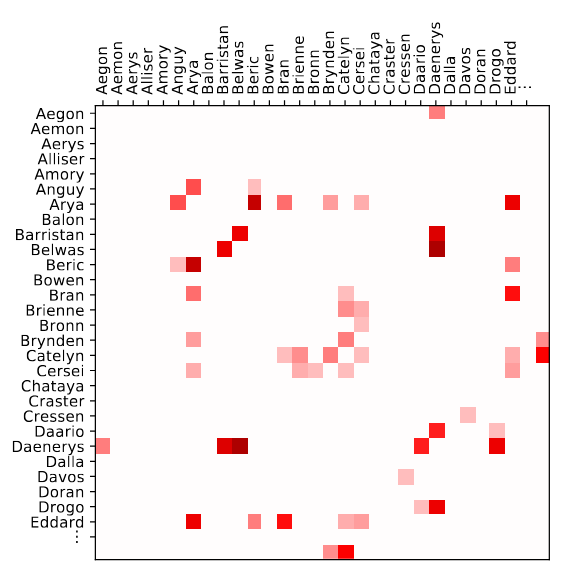
\includegraphics[scale=0.4]{got.png}
	\end{center}
\end{example}

The strengths of this type of visualization are that a lot of \textbf{qualitative information} can be gathered and it's really helpful for spotting \textbf{missing values} or \textbf{lack of normalization} before a more advanced data analysis.\\
At the same time, it gets quickly \textbf{overwhelming} with large datasets and it's \textbf{not very precise} about the values and their distribution.
\newpage
\subsubsection{Histograms}
This type of visualization focuses on just one feature so that more information can be extracted. The values are indicated by the position on the $x$-axis while the number of instances for each feature by the position on the $y$-axis.

\begin{example}[UCI Wholesale]
	In this example we have one Histogram for each product. Since there are different levels of spending, the result shows mainly the large spenders. To avoid this we apply the following \textbf{preprocessing}:
	\begin{equation*}
		z = \log(1+x)
	\end{equation*}
	and \textbf{standardization} (subtract the mean and divide by standard deviation).
	\begin{center}
		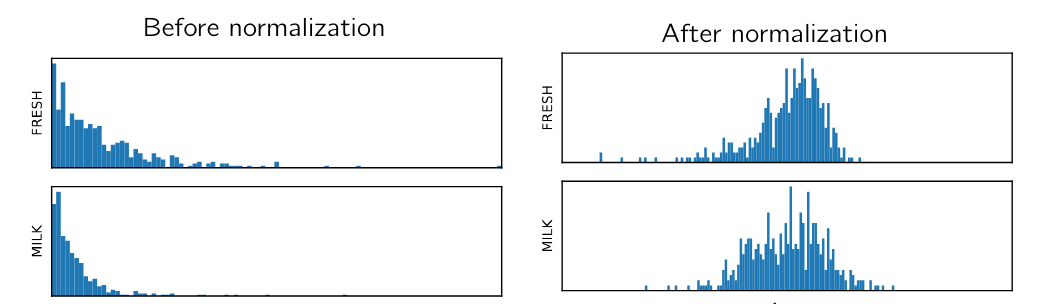
\includegraphics[scale=0.3]{histogram.png}
	\end{center}
\end{example}

Histograms are very \textbf{precise} in characterizing the distribution of individual features but they do not highlight correlations between them. Also, not practical with a high-dimensional dataset since we would need an Histogram for every feature.

\subsubsection{Scatter plots}
Scatter plots consider two features (on the axis) at the same time to find correlations. To improve them we can use \textbf{transparency} and build a black \textbf{outline} to better find outliers.

\begin{example}
	A scatter plot with the same dataset of the last example:
	\begin{center}
		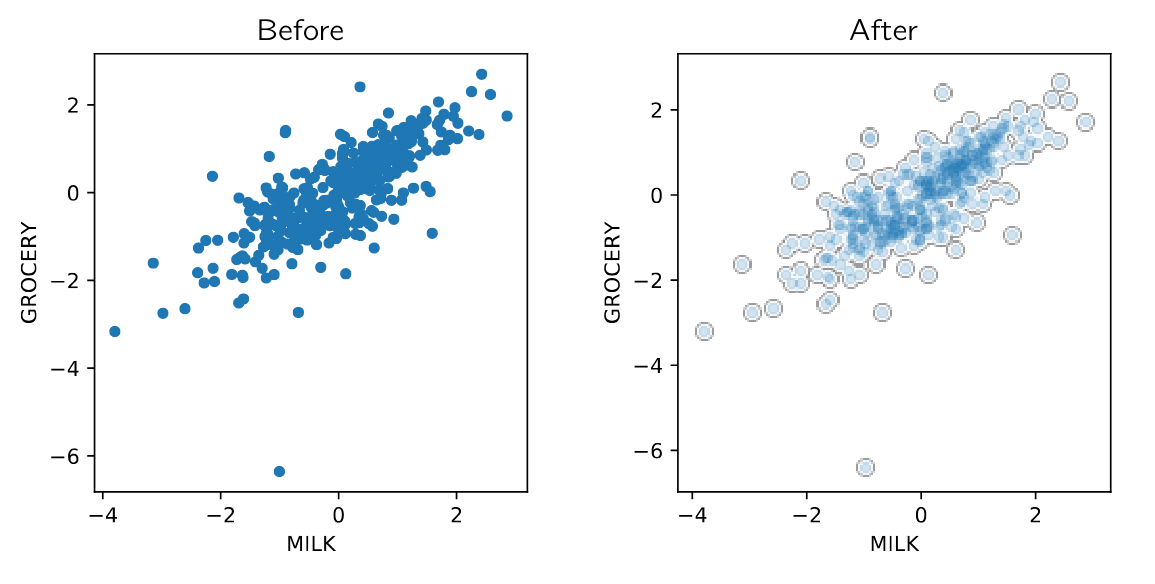
\includegraphics[scale=0.3]{scatter.png}
	\end{center}
\end{example}

\subsubsection{Graph visualization}
To visualize a graph, we arrange the nodes in a two-dimensional layout (e.g. a ring) and we draw lines between the nodes connected by an edge. If the edge strength is a real value, draw the line only if above a certain threshold.\\
It works well with a \textbf{sparse} graph.

\newpage
\begin{example}
	A \textbf{chord plot}, where the line used for each pair of nodes $(x_i, x_j)$ is the following parameterized curve
	\begin{equation}
		x(t) = x_i\cdot p^t + x_j\cdot (1-t)^p
	\end{equation}
	which is a line when $p=1$, otherwise it's a curve attracted to the center, making connections between nearby nodes more visible.
	\begin{center}
		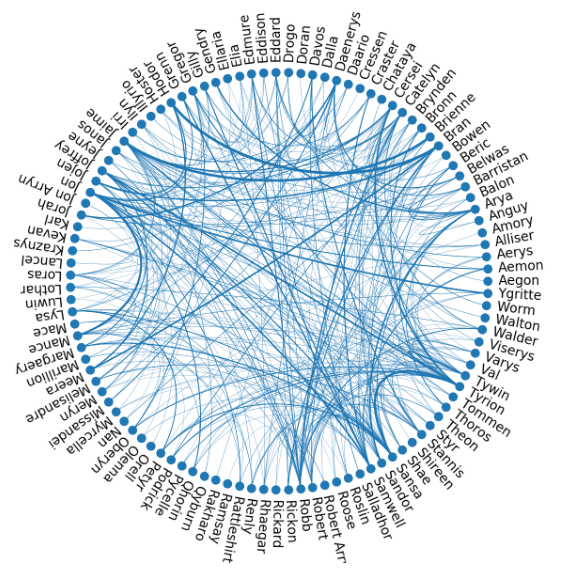
\includegraphics[scale=0.3]{chordplot}
	\end{center}
\end{example}

\subsection{Low dimensional embedding}
Low-dimensional embedding aims to construct a \textit{scatter plot} where the axes do not carry specific meaning but it's the \textbf{distance} that represent distances and similarities in the original input space.

\paragraph{Gradient descent}
Assuming you want to find the minimum of a function $J(\theta)$, follow:
\begin{enumerate}
	\item Initialize $\theta$ with a random value
	\item Apply repeatedly 
	\begin{equation}
		\theta \longleftarrow \theta - \gamma \bigtriangledown_\theta J(\theta)
	\end{equation}
	Where $\gamma$ is the \textbf{learning rate} set  appropriately to avoid slowing down the convergence or create instability.
	\item Return $\theta$
\end{enumerate}
\begin{note}
	\textbf{Initialization} is important to reach a good minimum. Gradient descent can be made to converge quickly by following the direction of the \textbf{average} of past gradients.
\end{note}

\subparagraph{Chain rule} Suppose that a \textbf{parameter of interest} $\theta_q$ (one element of the vector) is linked to $z$ through a mapping
\begin{equation*}
	\theta_q \longrightarrow a \longrightarrow b \longrightarrow z
\end{equation*}
then the derivative of the parameter of interest is the product of the local derivatives along the path
\begin{equation*}
	\frac{\delta z}{\delta \theta_q} = \frac{\delta z}{\delta b} \cdot \frac{\delta b}{\delta a} \cdot \frac{\delta a}{\delta \theta_q}
\end{equation*}
In practice the parameter of interest could be linked to the output through multiple paths. The rule is therefore extended by enumerating all the paths:
\begin{equation*}
	\frac{\delta z}{\delta \theta_q} = \sum_i \sum_j \frac{\delta z}{\delta b_j} \cdot \frac{\delta b_j}{\delta a_i} \cdot \frac{\delta a_i}{\delta \theta_q}
\end{equation*}

\subsubsection{MDS}
Multi Dimensional Scaling (MDS) is a low-dimensional embedding technique that generates for each instance a \textbf{vector} in low dimensions. These vectors are optimized so that the distances between points in low-dimensional space replicate the true distances between corresponding instances.\\
It follows this notation:
\begin{itemize}
	\item $d_{ij}$: \textbf{true distance} between the two instances, usually the Euclidean distance in the input space
	\begin{equation*}
		d_{ij} = \lvert\lvert x_i - x_j \rvert\rvert
	\end{equation*}
	\item $y_i$:  representation of the \textbf{instance} in low dimensional space (usually two dimensions)
	\item $\hat{d}_{ij}$: \textbf{distance} between the two instances in the low-dimensional space
	\begin{equation*}
		\hat{d}_{ij} = \lvert\lvert y_i - y_j \rvert\rvert
	\end{equation*}
\end{itemize}

\paragraph{Metric MDS}
It finds the embedding that minimizes the discrepancy between $d_{ij}$ and $\hat{d}_{ij}$ by minimizing
\begin{equation}
	\text{stress}(y_1, \ldots, y_N) = \bigg(\frac{\sum_{i<j}(d_{ij} - \hat{d}_{ij})^2}{\sum_{i<j}d^2_{ij}}\bigg)^\frac{1}{2}
\end{equation} 
The idea is similar to connecting the data points with strings, each one with a specific length in a relaxed state, which is determined by the input space. The Metric MDS solution is given by the relaxed state of the spring system.

\begin{center}
	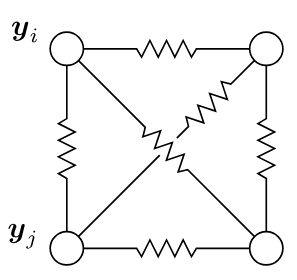
\includegraphics[scale=0.3]{mds}
\end{center}

The algorithm starts with a random initialization of the points $y_1, \ldots, y_N$ and iteratively updates them to minimize the \textit{stress} function. The optimization procedure is usually done multiple times with different seeds.\\
Another technique is with the \textbf{gradient descent}, considering a slightly different stress function
\begin{equation}
	\text{stress}(y) = C \cdot \big(\sum_{i<j} ( \Delta_{ij} - d_{ij})^2\big)^\frac{1}{2} \qquad\qquad \Delta_{ij} = \lvert\lvert y_i - y_j \rvert\rvert 
\end{equation}
and with the gradient given by
\begin{equation}
	\frac{\delta_{\text{stress}}}{\delta_{y_k}} = C \cdot \sum_{i<j} \frac{\Delta_{ij}}{\lvert\lvert \Delta \rvert\rvert} \cdot \frac{y_i - y_y}{\lvert\lvert y_i - y_j \rvert\rvert} \cdot (\delta_{ik} - \delta_{jk}) \qquad\qquad \Delta = (\Delta_{ij})_{i<j}
\end{equation}

\paragraph{Non Metric MDS}
Extends Metric MDS with the application of a fine transformation $f$ (learnt from data) to the distances. This allows for handling mismatches, enabling points that are relatively close in space to be very close in embedded space and points that are relatively far in space to be very far in embedded space.
\begin{equation}
	\text{stress}(y_1, \ldots, y_N) = \bigg(\frac{\sum_{i<j}(d_{ij} - f(\hat{d}_{ij}))^2}{\sum_{i<j}d^2_{ij}}\bigg)^\frac{1}{2}
\end{equation} 
\newpage
\paragraph{Comparison} Non Metric MDS matches more faithfully true distances between data points (up to an affine transformation) and appears crowded near the center of the visualization.
\begin{figure}[!h]
	\hfill
	\subfigure[Metric MDS]{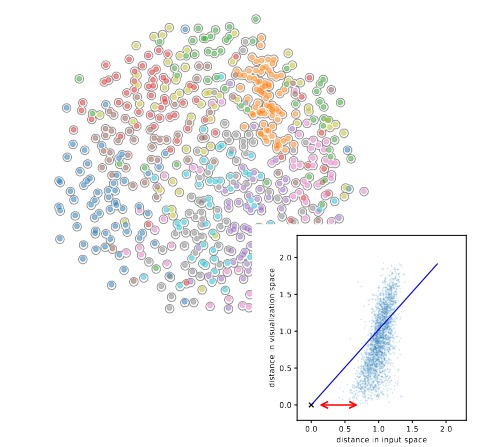
\includegraphics[scale=0.4]{mmds}}
	\hfill
	\subfigure[Non Metric MDS]{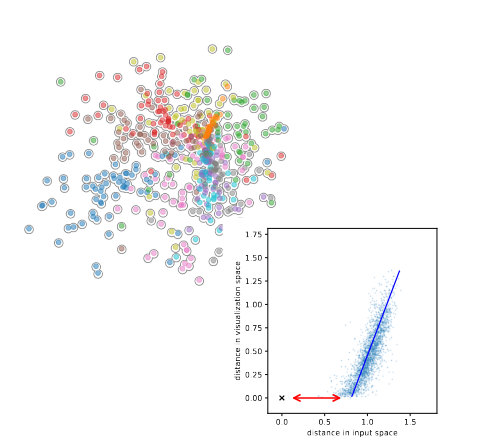
\includegraphics[scale=0.4]{nmds}}
	\hfill
\end{figure}

\subsubsection{T-SNE}
This method ensures to preserve \textbf{similarities}, promoting a correct representation of small distances and tolerating large errors for large distances.\\
It aims to learn embedding coordinates such that similarities between points matches similarities in embedded space. The collection of pairwise \textbf{similarities} are viewed as two probabilities distribution defined over the pair of points: $p$ in the \textit{input space} and $q$ in the \textit{embedded space}.\\
The embedding $\mathbf{y} = (\mathbf{y}_1, \ldots, \mathbf{y}_N)$ is such that minimizes the KL divergence
\begin{equation}
	D_{KL}(p \vert\vert q(\mathbf{y})) = \sum_{ij} p_{ij} \log\frac{p_{ij}}{q_{ij}(\mathbf{y})}
\end{equation}
This function is minimized through \textbf{gradient descent}:
\begin{equation*}
	\mathbf{y} \longleftarrow y - \gamma \cdot \bigtriangledown D_{KL}(p \vert\vert q(\mathbf{y}))
\end{equation*}

\paragraph{Modeling} Similarities are modeled using different functions for the input and the embedded space because of the \textbf{concentration of distances}.

\begin{definition}[Concentration of distances]
	The squared Euclidean distance between two points is given as a sum over individual dimensions:
	\begin{equation}
		\lvert\lvert \mathbf{x} - \mathbf{x}' \rvert\rvert ^ 2 = \sum_{t=1}^{d} (x_t - x_t')^2
	\end{equation}
	Assuming dimensions-wise squared distances are iid. (e.g. random data), the expected square distance grows linearly with $d$ but the standard deviation grows with $\sqrt{d}$ (cf. law of large numbers).
	\begin{center}
		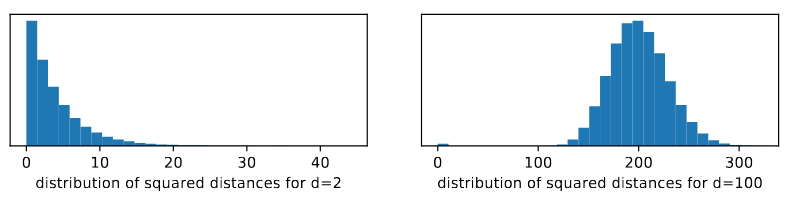
\includegraphics[scale=0.3]{concdist}
	\end{center}
\end{definition}
\newpage
Similarities $p_{ij}$ in the \textbf{input space} are modeled with the \textbf{Gaussian} function
\begin{equation}
	p_{ij} = \frac{1}{Z} \exp\big(- \frac{\lvert\lvert \mathbf{x}_i - \mathbf{x}_j \rvert\rvert^2}{2 \sigma^2}\big)
\end{equation}
with $Z$ being a normalizing term that ensures $\sum_{ij} p_{ij}=1$. The scale $\sigma$ is determined by another parameter called \textbf{perplexity}.

\begin{note}
	In practice, to better represent low connectivity regions, one first computes conditional distributions $p_{i \vdash j}$ and $p_{j \vert i}$ and then sets $p_{ij} \propto p_{i \vert j} + p_{j \vert i}$.
\end{note}
Similarities $q_{ij}$ in the \textbf{embedded} space are modeled with the \textbf{t-Student} function
\begin{equation}
	q_{ij}(\mathbf{y}) = \frac{1}{Z} \cdot \frac{1}{1+ \lvert\lvert \mathbf{y}_i - \mathbf{y}_j \rvert\rvert^2}
\end{equation}
with $Z$ set such that $\sum_{ij}q_{ij}=1$.

\paragraph{Early exaggeration} It's the initial phase of T-SNE where the gradient of the objective
\begin{equation}
	\bigtriangledown D_{KL}(p \vert\vert q(\mathbf{y})) = 4 \cdot \sum_{j}(p_{ij}-q_{ij})\cdot \frac{\mathbf{y}_i - \mathbf{y}_j}{1+\lvert\lvert \mathbf{y}_i - \mathbf{y}_j\rvert\rvert^2}
\end{equation}
is modified by multiplying the values $p_{ij}$ by a factor $\alpha$ in the gradient computations. The optimization loses its probabilistic phase but it helps to escape the local optima and build compact clusters in embedded space representing	 the cluster structure of the input data.

\subsubsection{Comparison}
T-SNE better resolves the local structures of the data and identifies \textbf{clusters}, while MDS better preserves overall distances.
\begin{figure}[!h]
	\hfill
	\subfigure[MDS]{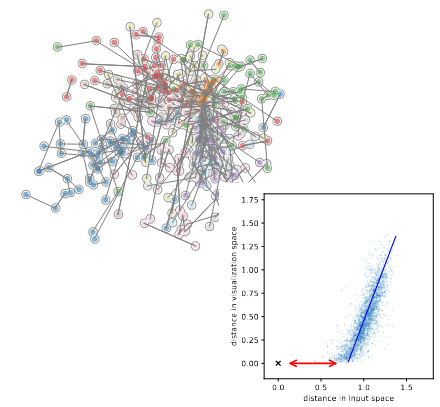
\includegraphics[scale=0.4]{mds2}}
	\hfill
	\subfigure[T-SNE]{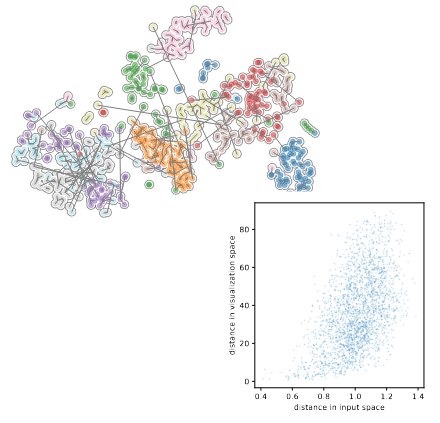
\includegraphics[scale=0.4]{tsne}}
	\hfill
\end{figure}

\subsubsection{Networks}
Usually embedding techniques are used for tabular data but they might also be used for \textbf{network data} (e.g. adjacency matrix). There are different approaches:
\begin{itemize}
	\item Use an embedding techniques that natively works with adjacencies
	\item Consider the adjacency matrix as a data matrix $X \leftarrow A$
	\item Cholesky decomposition $A = LL^T$ and then $X \leftarrow L$
\end{itemize}

\begin{example}
	Embedding of the Game of Thrones relationships.
	\begin{center}
		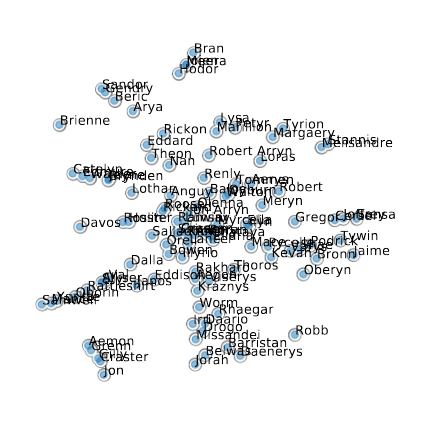
\includegraphics[scale=0.3]{got2}
	\end{center}
\end{example}

\subsubsection{Stringing}
Visualizing the data as an array can be overwhelming when the number of instances and dimensions is large. We can apply \textbf{T-SNE} to the dataset and observe that the embedding coordinates define an \textbf{ordering of instances}. We can the redraw the matrix according to it, getting an easier to interpret visualization.

\begin{figure}[!h]
	\hfill
	\subfigure[Before]{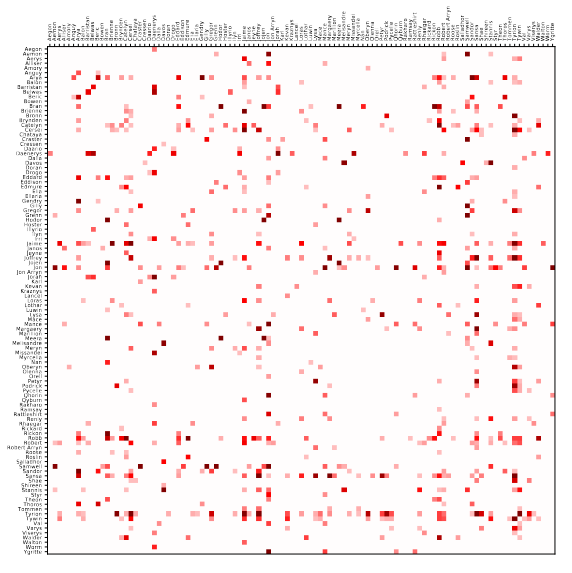
\includegraphics[scale=0.3]{str1}}
	\hfill
	\subfigure[After]{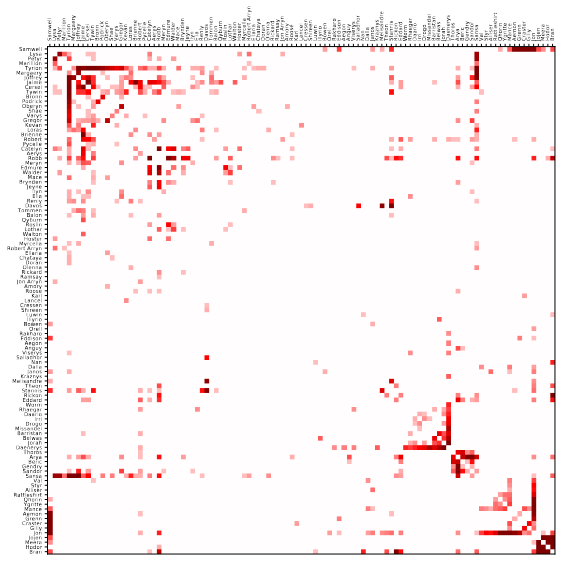
\includegraphics[scale=0.3]{str2}}
	\hfill
\end{figure}

\subsubsection{Limits}
Low-embedding techniques have two main problems:
\begin{itemize}
	\item They could find structures that in reality do not exist
	\item They can distort the geometry of the input data 
\end{itemize}
% !TeX spellcheck = en_US
\newpage
\section{Data dispersion}
Dispersion is an important property of the data that indicates how much \textbf{variation} there is in some dataset $D=(\mathbf{x_1, \ldots, \mathbf{x}_N})$. There are various possible measures:
\begin{itemize}
	\item \textbf{Number} of distinct \textbf{data points}
	\item \textbf{Radius} of minimal enclosing sphere
	\item \textbf{Average square Euclidean distance} from the dataset mean $\mathbf{m}$
	\begin{equation}
		s(X)=\frac{1}{N} \sum_{i=1}^{N}\lvert\lvert \mathbf{x}_i - \mathbf{m}\rvert\rvert^2
	\end{equation}
\end{itemize}
Often it's important also to describe the \textbf{structure} of dispersion.
\begin{center}
	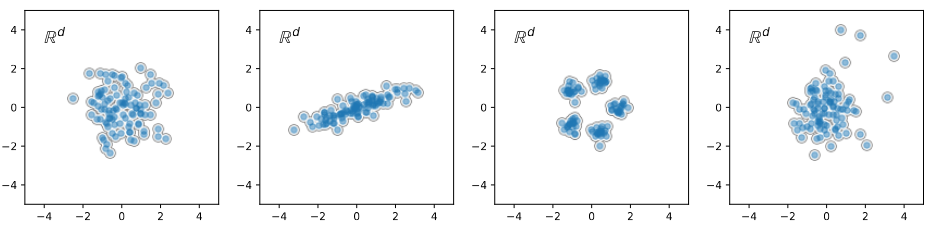
\includegraphics[scale=0.4]{disp}
\end{center}

\subsection{Lagrange multipliers}
The method of Lagrange multipliers is a general framework for finding solutions of constrained optimization problems of the type
\begin{equation*}
	\arg\max_\theta f(\theta) \qquad\qquad g(\theta)=0
\end{equation*}
It consists in the following steps:
\begin{enumerate}
	\item Construct the \textbf{Lagrangian}
	\begin{equation}
		\mathcal{L}(\theta, \lambda) = f(\theta) + \lambda \cdot g(\theta)
	\end{equation}
	where $\epsilon$ is the \textbf{Lagrangian multiplier}
	\item Solve the equation
	\begin{equation}
		\bigtriangledown\mathcal{L}(\theta, \lambda)=0
	\end{equation}
	This includes that the gradient of objective and constraint are aligned but point in opposite direction:
	\begin{equation}
		\bigtriangledown f(\theta) = -\lambda\bigtriangledown g(\theta)
	\end{equation}
\end{enumerate}

\subsection{PCA}
Principal Component Analysis is a specific type of dispersion which can\\ be described in terms of \textbf{directions} in input space.\\
\begin{wrapfigure}[10]{r}{4cm}
	\vspace{-2.5cm}
	\begin{center}
		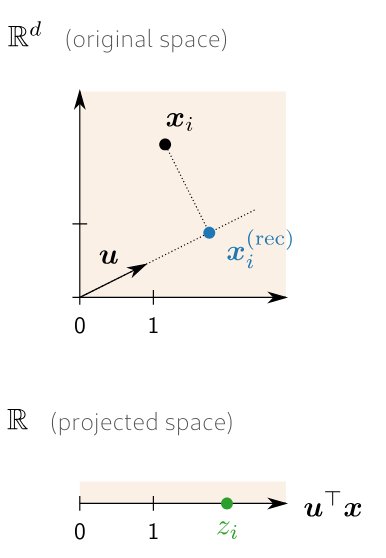
\includegraphics[width=4cm]{pca1}
	\end{center}
\end{wrapfigure}
We start with the following \textbf{preliminaries}:
\begin{itemize}
	\item Let $\mathbf{x}_1, \ldots, \mathbf{x}_N \in \mathbb{R}^d$ be a \textbf{dataset}, where $d$ is the number of \textbf{input features} and $N$ is the number of \textbf{data points}
	\item Let $u \in \mathbb{R}^d$ be a vector of same dimensions, that represents some \textbf{directions} in the input space and is constrained to be of norm $\lvert\lvert u \rvert\rvert = 1$
	\item Data points can be \textbf{projected} onto the direction via the dot product
	\begin{equation}
		\forall_{i=1}^N : z_i = \mathbf{u}^T \mathbf{x}_i
	\end{equation}
	\item The projections can be \textbf{backprojected} on the input space by doing the dot product once again
	\begin{equation}
		\forall_{i=1}^N: \mathbf{x}_i^{\text{(rec)}} = \mathbf{u}\mathbf{u}^T \mathbf{x}_i
	\end{equation}
\end{itemize}
\subsubsection{Formulations}
We have two possible formulations:
\paragraph{Dispersion maximization} Find a projection $z = \mathbf{u}^T \mathbf{x}$ of the data under which the dispersion (variance) is maximized.\\
This means finding a direction $\mathbf{u}$ (with $\lvert\lvert \mathbf{u} \rvert\rvert = 1$) so that the data projected onto this direction $z_1, \ldots, z_N$ has maximum variance.
\begin{equation}
	\arg\max_\mathbf{u} \big[\frac{1}{N} \sum_{i=1}^N(\mathbf{u}^T\mathbf{x}_i-\tilde{m})^2\big] \qquad\qquad \mathbf{u}^T\mathbf{x}_i = z_i
\end{equation}
where $\tilde{m} = \frac{1}{N} \sum_{i=1}^Nz_i$ is the dataset mean in the projected space. \underline{Since we center the data}, we then have $\tilde{m}=0$ and therefore
\begin{equation}
	\label{eq:dispmax}
	\arg\max_\mathbf{u} \big[\frac{1}{N} \sum_{i=1}^N(\mathbf{u}^T\mathbf{x}_i)^2\big]
\end{equation}
\paragraph{Error minimization} Find the direction that minimizes the reconstruction error (MSE) between the original data point $\mathbf{x}$ and its backprojection $\mathbf{x}^{\text{(rec)}} = \mathbf{u}\mathbf{u}^T\mathbf{x}$.\\
This means finding the direction $\mathbf{u}$ (with $\lvert\lvert \mathbf{u} \rvert\rvert = 1$) so that the data projected on the corresponding subspace best reconstructs the original data, having \textbf{minimal squared distance} to it.
\begin{equation}
	\arg\min_\mathbf{u}\big[\frac{1}{N}\sum_{i=1}^N \lvert\lvert \mathbf{x}_i - \mathbf{u}\mathbf{u}^T\mathbf{x}_i\rvert\rvert^2\big] \qquad\qquad \mathbf{u}\mathbf{u}^T\mathbf{x}_i = \mathbf{x}_i^{\text{(rec)}}
\end{equation}

\begin{observation}
	As of Pearson 1901, the two views coincide:
	\begin{align*}
		& \arg\min_\mathbf{u}\big[\frac{1}{N}\sum_{i=1}^N \lvert\lvert \mathbf{x}_i - \mathbf{u}\mathbf{u}^T\mathbf{x}_i\rvert\rvert^2\big]\\
		& = \arg\min_\mathbf{u}\big[\frac{1}{N}\sum_{i=1}^N (\mathbf{x}_i - \mathbf{u}\mathbf{u}^T\mathbf{x}_i)^T(\mathbf{x}_i - \mathbf{u}\mathbf{u}^T\mathbf{x}_i)\big] \\
		& = \arg\min_\mathbf{u}\big[\frac{1}{N}\sum_{i=1}^N \mathbf{x}_i^T\mathbf{x}_i - 2\mathbf{x}_i^T\mathbf{u}\mathbf{u}^T\mathbf{x}_i+(\mathbf{u}\mathbf{u}^T\mathbf{x}_i)^T(\mathbf{u}\mathbf{u}^T\mathbf{x}_i)\big] \\
		& = \arg\min_\mathbf{u}\big[\frac{1}{N}\sum_{i=1}^N -2(\mathbf{x}_i^T\mathbf{u})^2+\mathbf{x}_i^T\mathbf{u}\mathbf{u}^T\mathbf{u}\mathbf{u}^T\mathbf{x}_i\big] \\
		& = \arg\min_\mathbf{u}\big[\frac{1}{N}\sum_{i=1}^N -2(\mathbf{x}_i^T\mathbf{u})^2+(\mathbf{x}_i^T\mathbf{u})^2\big]\\
		& = \arg\max_\mathbf{u} \big[\frac{1}{N} \sum_{i=1}^N(\mathbf{u}^T\mathbf{x}_i)^2\big]
	\end{align*}
	\begin{figure}[!h]
		\hfill
		\subfigure[Error minimization]{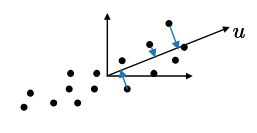
\includegraphics[scale=0.3]{pcamin}}
		\hfill
		\subfigure[Dispersion maximization]{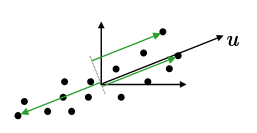
\includegraphics[scale=0.3]{pcamax}}
		\hfill
	\end{figure}
\end{observation}
\subsubsection{Solution}
To find the principal component, we start from the dispersion maximization equation \ref{eq:dispmax} and rewrite it as
\begin{align*}
	& \arg\max_\mathbf{u} \big[\frac{1}{N} \sum_{i=1}^N(\mathbf{u}^T\mathbf{x}_i)^2\big] \\
	& = \arg\max_\mathbf{u} \big[\frac{1}{N} \sum_{i=1}^N (\mathbf{u}^T\mathbf{x}_i)(\mathbf{x}_i^T\mathbf{u})\big]\\
	& = \arg\max_\mathbf{u} \big[\mathbf{u}^T \big(\frac{1}{N} \sum_{i=1}^N\mathbf{x}_i\mathbf{x}_i^T\big)\mathbf{u}\big] \qquad\qquad \lvert\lvert u \rvert\rvert = 1
\end{align*}
where $\Sigma = \frac{1}{N} \sum_{i=1}^N\mathbf{x}_i\mathbf{x}_i^T$ is the \textbf{covariance matrix} that, since it does not depend on $\mathbf{u}$, can be precomputed. We apply the Lagrangian multipliers method:
\begin{enumerate}
	\item We rewrite the constraint as $\lvert\lvert u \rvert\rvert^2 = 1$ and build the Lagrangian
	\begin{equation*}
		\mathcal{L}(\mathbf{u}, \lambda) = \mathbf{u}^T \Sigma\mathbf{u} + \lambda \cdot (1-\lvert\lvert \mathbf{u} \rvert\rvert ^2)
	\end{equation*}
	\item We set the gradient to zero
	\begin{align*}
		& \nabla_\mathbf{u}\mathcal{L}(\mathbf{u}, \lambda)=0 \Rightarrow \Sigma\mathbf{u}=\lambda\mathbf{u} \\
		& \nabla_\lambda\mathcal{L}(\mathbf{u}, \lambda)=0 \Rightarrow \lvert\lvert \mathbf{u}\rvert\rvert^2=1
	\end{align*}
	This means that the solution is an \textbf{eigenvector} of $\Sigma$, in particular
	\begin{align*}
		& \Sigma\mathbf{u}=\lambda\mathbf{u}  \\
		& \mathbf{u}^T\Sigma\mathbf{u}=\lambda\mathbf{u}\mathbf{u}^T \\
		 & \mathbf{u}^T\Sigma\mathbf{u}=\lambda\\
	\end{align*}
	meaning that for the \textit{objective} (left part of the equation) to be maximized, we have to choose the eigenvector in a way that the corresponding eigenvalue $\lambda$ is maximum, therefore the \textbf{leading eigenvector}.
\end{enumerate}
\subsubsection{Problems} The major problems are:
\begin{itemize}
	\item PCA is not very robust to \textbf{outliers}. We need to clean the data before.
	\item PCA does not describe well the data when it's strongly \textbf{non-Gaussian}. It fails to account for the fact that data may vary locally in different directions.
\end{itemize}
\newpage
\subsubsection{Multiple components}
The basic PCA method consists of rewriting the data as the sum of two components: what PCA is able to \textbf{reconstruct} and a \textbf{residue} of what cannot be captured.
\begin{equation}
	\mathbf{x}=\mathbf{u}\mathbf{u}^T\mathbf{x}+(\mathbf{x}-\mathbf{u}\mathbf{u}^T\mathbf{x})
\end{equation}
It's possible to find secondary principal components in the residue with the following algorithm:
\begin{lstlisting}[mathescape=true]
	$X_{\text{res}} \leftarrow X$
	for j=1 to h do
		$w_j \leftarrow \text{PCA}(X_{\text{res}})$
		$X_{\text{res}} \leftarrow X_{\text{res}} -\mathbf{w}_j \mathbf{w}_j^TX_{\text{res}}$
	end for 
\end{lstlisting}
This gives as output a collection of directions $w_1, \ldots, w_h$ which are called the \textbf{principal components}.

\begin{observation}
	The principal components are equivalent to the eigenvectors $\mathbf{u}_1, \ldots, \mathbf{u}_h$ of the covariance matrix $\Sigma$ sorted by decreasing associated eigenvalues $\lambda_1 > \lambda_2 > \ldots > \lambda_h$.\\
	It's therefore sufficient to compute all eigenvectors and eigenvalues of $\Sigma$ and then sort them to get the full solution of PCA.
\end{observation}

\subsubsection{Biplot}
The biplot is a common visualization on the two leading principal components. Each instance corresponds to a point in a scatter plot and its coordinates are given by the pair
\begin{equation*}
	(\mathbf{u}_1^T\mathbf{x}, \mathbf{u}_2^T\mathbf{x})
\end{equation*}
Input features can also be visualized in this plot by projecting their associate canonical coordinate vector in PCA space. They are usually depicted as arrows with the feature name and rescaled for visualization purposes.
\begin{center}
	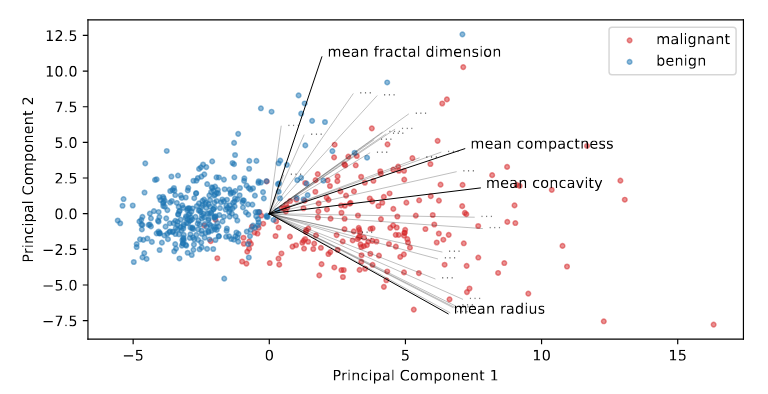
\includegraphics[scale=0.4]{biplot}
\end{center}

\subsubsection{Explained variance}
The \textbf{dispersion} of a multivariate set can be measured as the generalized variance, which can be expressed in therms of $\Sigma$:
\begin{equation}
	s_{\text{tot}}=\mathbb{E}[\lvert\lvert \mathbf{x} - \mathbf{m}\rvert\rvert^2] = \sum_{j=1}^{d} \mathbb{E}[(x_{ij}-m_j)^2] = \text{Tr}(\Sigma)
\end{equation}
where $\mathbb{E}[\cdot]$ denotes an average over points in the dataset.\\
The variation of the data projected on the $k$th principal component can be expressed as
\begin{equation}
	s_k = \mathbb{E}[(\mathbf{u}_k^T(\mathbf{x}-\mathbf{m}))^2] = \mathbf{u}_k^T\Sigma\mathbf{u}_k=\lambda_k
\end{equation}
meaning that it corresponds to the $k$th eigenvalue of the covariance matrix. Therefore the following is true:
\begin{equation}
	\text{Tr}(\Sigma) = \sum_{k=1}^{h}\lambda_k
\end{equation}
This means that PCA produces an additive \textbf{decomposition} of the total dispersion in terms of principal components.
\begin{center}
	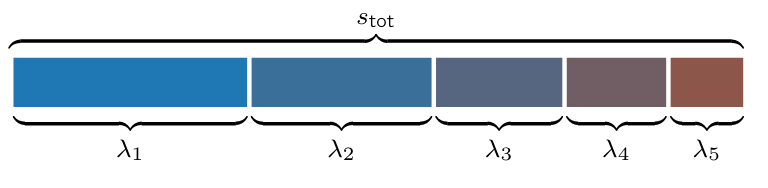
\includegraphics[scale=0.4]{pcadecomp}
\end{center}

\begin{example}
	We could have three two dimensional datasets that have the same overall dispersion $s_\text{tot}$ but distributed differently over principal components:
	\begin{center}
		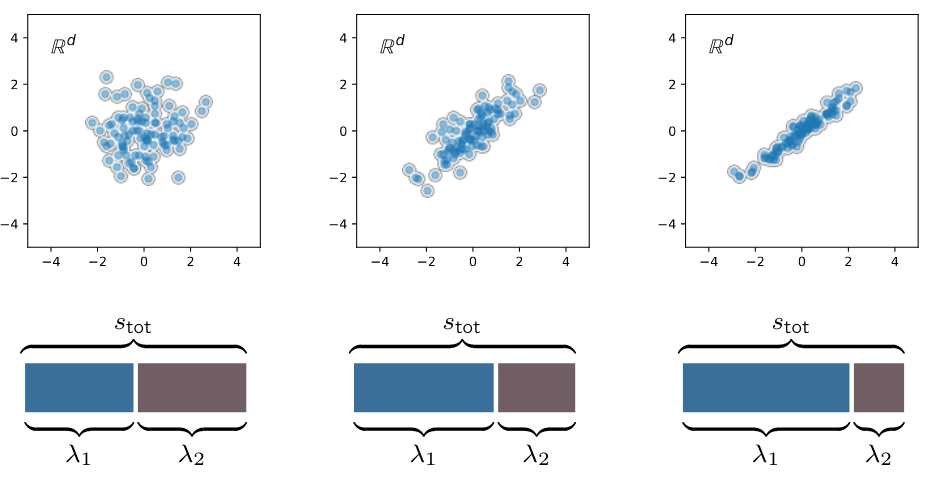
\includegraphics[scale=0.4]{pcaex}
	\end{center}
\end{example}

\subsubsection{Scree plot}
The scree plot is useful to get a picture of the effective \textbf{dimensionality of the data}. If only the first few bars are large, it means that the effective dimensionality is small and the data is simple.
\begin{center}
	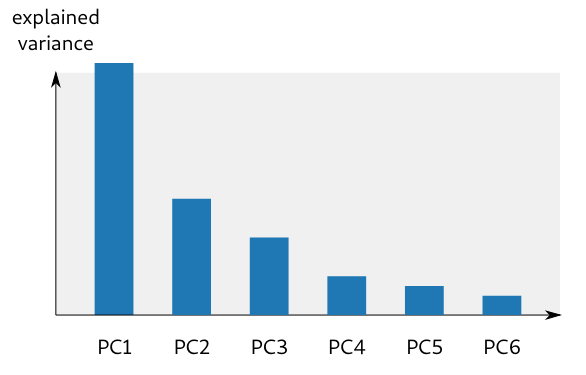
\includegraphics[scale=0.4]{scree}
\end{center}
In this plot, each bar corresponds to the \textit{explained variance} associated to a particular principal component. Its height is given by the associated \textit{eigenvalue}. It can be interpreted as the share of the total variance explained by this component.
\begin{note}
	Sometimes the information is better depicted as a \textbf{cumulative plot} where the $k$th bar indicates the variance obtained retaining the leading $k$ principal components.
\end{note}

\subsubsection{Applications}
PCA is not used only to describe the data but also to remove certain factors that contribute to data dispersion, such as:
\begin{itemize}
	\item \textbf{Artifact} removal: it may be reasonable to remove first principal components (e.g. eye blinking in EEG)
	\item \textbf{Denoising}: remove last principal components
\end{itemize}
\subsubsection{Improvements}
Since many data are high-dimensional, the standard implementation of the PCA would have to compute a covariance matrix $\Sigma$ of $d \times d$ size, which would be time and space consuming.
\paragraph{SVD}
\begin{definition}[SVD]
	A singular value decomposition factorizes a matrix $M = U \Lambda V$ where
	\begin{itemize}
		\item $U$ contains the eigenvectors of $MM^T$
		\item $V$ contains the eigenvectors of $M^TM$
		\item $\Lambda$ is a diagonal matrix, with diagonal elements of $\Lambda^2$ containing the eigenvalues of $MM^T$
	\end{itemize}
\end{definition}
Since SVD extracts the eigenvectors and eigenvalues of the matrix $MM^T$ and PCA solutions corresponds to those of the covariance matrix $\Sigma$, we can compute the latter by setting $\Sigma = MM^T$, therefore
\begin{equation}
	M = \frac{1}{\sqrt{N}}X
\end{equation}
The \textbf{algorithm} is the following:
\begin{enumerate}
	\item Let $X$ be our data matrix of size $d \times N$
	\item Define $M = \frac{1}{\sqrt{N}}X$
	\item Feed the matrix $M$ to SVD and get $U$, $\Lambda$ and $V$
	\item PCA eigenvectors are the columns of $U$ while eigenvalues are the diagonal elements of $\Lambda^2$
\end{enumerate}
When computing the matrix $U$ we have the option to not calculate all the matrices, which for $d>N$ would be a huge amount. In that case $U$ is $d \times N$.\\
The \textbf{complexity} of the algorithm is $O(\min(N^2d,d^2N))$, but when $d \approx N$, it becomes as bad as the one for computing the eigenvectors of $\Sigma$ ($O(d^3)$).

\paragraph{Power Iteration} Since in large datasets even SVD is prohibitive and often we just need the first principal components, we can use the power iteration algorithm to get them. The following finds the \textbf{first} principal component:
\begin{lstlisting}[mathescape=true]
	$u \approx$ random()
	repeat
		$v \leftarrow \Sigma \mathbf{u}$
		$\mathbf{u} \leftarrow \frac{\mathbf{v}}{\lvert\lvert \mathbf{v} \rvert\rvert}$
	until convergence
\end{lstlisting}
It \textbf{always} converges \textbf{exponentially fast}.\\
To get the following ones:
\begin{lstlisting}[mathescape=true]
	$\Sigma = \frac{1}{N}XX^T$
	for j=1 to h do
		$\mathbf{u}_j \leftarrow \text{POWIT}(\Sigma)$
		$\Sigma \leftarrow \Sigma - \mathbf{u}_j \mathbf{u}_j^T\Sigma$
	end for
\end{lstlisting}
% !TeX spellcheck = en_US
\newpage
\section{Anomalies}
Anomalies are points that escape the models prediction capabilities. Hence, a model for anomaly detection should focus on the opposite of what's been predicted to be normal.

\begin{example}
	An example application is when discovering anomalous or rare geological properties for resource monitoring and extraction.
\end{example}

\subsection{Classical}
\subsubsection{Z-score}
The Z-score is a common measure of anomalies in statistical studies.
\begin{equation}
	z = \frac{(x - \mu)}{\sigma}
\end{equation}
Where $\mu$ is the \textit{mean} and $\sigma$ the \textit{standard deviation}.
\begin{center}
	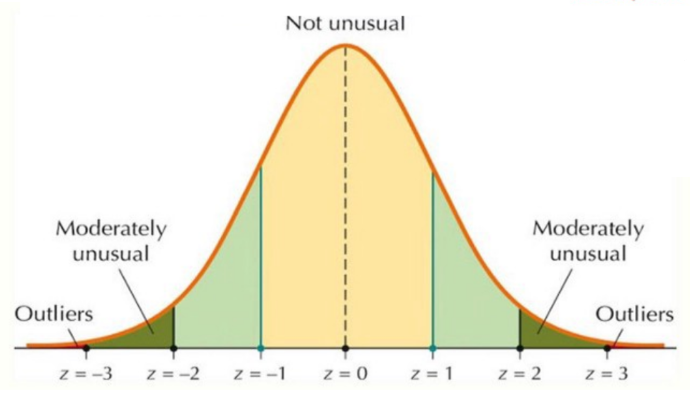
\includegraphics[scale=0.3]{zscore}
\end{center}
Points can be considered outliers if their z-score is above a certain threshold, usually $\lvert z \rvert > 3$.

\begin{observation}
	When input feature are correlated (\textbf{multivariate data}), z-score of individual features cannot properly detect outliers.
\end{observation}

\subsubsection{Mahalanobis Distance}
The Mahalanobis Distance is the generalization of the concept of the z-score. It defines how many standard deviations the model is away from the center of the data, taking into account \textbf{correlations}. \\\\
The Mahalanobis Distance of a point $x \in \mathbb{R}^d$ to a reference distribution of mean $\mu \in \mathbb{R}^d$ and covariance $\Sigma\in \mathbb{R}^{d\times d}$ is defined as:
\begin{equation}
	z=\sqrt{(x-\mu)^T \Sigma^{-1}(x-\mu)}
\end{equation}
\begin{center}
	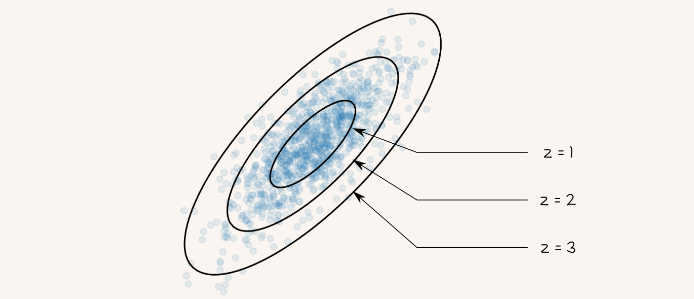
\includegraphics[scale=0.3]{md}
\end{center}

We can relate the distance to the z-score computed in PCA space by the formula
\begin{equation}
	z = \sqrt{\sum_{j=1}^{d}(x_{\text{PCA}-j})^2}
\end{equation}

\paragraph{Limits} The main problem is that in high dimensions the matrix $\Sigma^{-1}$ tends to get \textbf{uncontrollably large} due to the correlations that arise from the limited data. This instability can be addressed by adding a small diagonal term to the covariance matrix, making the anomaly score more robust.
\begin{equation}
	\Sigma \leftarrow \Sigma+\epsilon I
\end{equation}
Furthermore, in presence of \textbf{skewed non-Gaussian} distribution, the Mahalanobis Distance does not describe well data.

\subsection{Boundary-Based}
The idea behind this method is to learn a geometrical object that encloses most of the data but the outliers. E.g. hyper sphere or polytope.
\begin{equation}
	\mathcal{O}(S,\mathbf{c}) = \{\mathbf{x} \in \mathbb{R}^d : h(\mathbf{x}, \mathbf{c}) \leq S\}
\end{equation}
Then we have to find a minimum enclosing object:
\begin{equation}
	\min_{S, \mathbf{c}, \mathbf{\varepsilon}} S+C\sum_{i=1}^{N}\varepsilon_i \qquad\qquad \forall_{i=1}^N : h(\mathbf{x}_i; \mathbf{c}) \leq S + \varepsilon_i \qquad\forall_{i=1}^N : 0 \leq \varepsilon_i
\end{equation}
Optimization problem with inequality constraints, like this one, can be studied within KKT conditions.

\subsubsection{KKT Conditions}
\begin{definition}[KKT Conditions]
	Given an optimization problem in the following form
	\begin{equation*}
		\min_\theta f(\mathbf{\theta}) \qquad\qquad \forall_{i=1}^M : g_i(\mathbf{\theta}) \leq 0
	\end{equation*}
	e defined the Lagrangian function
	\begin{equation*}
		\mathcal{L}(\mathbf{\theta}, \mathbf{\lambda}) = F(\mathbf{\theta}) + \sum_{i=1}^{M} \lambda_i g_i(\mathbf{\theta})
	\end{equation*}
	If $\mathbf{\theta}^*$ is a solution of the optimization problem, and the latter satisfies some regularity conditions (e.g. objective convex, all constraint convex and existence of $\mathbf{\theta}$ that satisfies them with strict inequalities), then exists a constant vector $\mathbf{\lambda}$ such that the solution satisfies:
	\begin{itemize}
		\item \textbf{Stationarity}
		\begin{equation}
			\nabla_\mathbf{\theta} \mathcal{L}(\mathbf{\theta^*}, \mathbf{\lambda}) = 0
		\end{equation}
		\item \textbf{Primal feasibility}
		\begin{equation}
			\forall_{i=1}^M : g_i(\mathbf{\theta^*}) \leq 0
		\end{equation}
		\item \textbf{Dual feasibility}
		\begin{equation}
			\forall_{i=1}^M:\lambda_i \geq 0
		\end{equation}
		\item \textbf{Complementary slackness}
		\begin{equation}
			\forall_{i=1}^M: \lambda_i g_i(\mathbf{\theta^*}) = 0
		\end{equation}
	\end{itemize}
\end{definition}

KKT conditions provide a set of equation with a solution $\mathbf{\theta^*}$ needs to satisfy. Usually they cannot be solved analytically and thus optimization is needed. There are two approaches:
\begin{itemize}
	\item \textbf{Primal}: solve the optimization problem
	\begin{equation}
		\min_\mathbf{\theta} f(\mathbf{\theta}) \qquad\qquad \forall_{i=1}^M: g_i(\mathbf{\theta}) \leq 0
	\end{equation}
	\item \textbf{Lagrange Dual}: the idea is to penalize constraint violations directly into the objective
	\begin{equation}
		\max_{\mathbf{\lambda}\succeq 0} \inf_\mathbf{\theta} \big\{f(\mathbf{\theta}) + \sum_{i=1}^{M} \lambda_i g_i(\mathbf{\theta})\big\}
	\end{equation}
	Then the primal parameters $\mathbf{\theta^*}$ can be recovered from the dual solution $\mathbf{\lambda}^*$ using KKT conditions.
\end{itemize}

\subsection{SVDD}
Support Vector Data Description requires the building of a hyper sphere
\begin{equation}
	\mathcal{H} = \{\mathbf{x} \in \mathbb{R}^d: \lvert\lvert \mathbf{c} - \mathbf{x} \rvert\rvert^2 = S\}
\end{equation}
with parameters $(\mathbf{c}, S)$ where $S=R^2$ is a variable modeling the square radius. They are chosen in a way that encloses most data points and has minimum radius.\\
Points should be included in $\mathcal{H}$, however to account fo anomalies, one allows points to be outside with a \textbf{penalty} $\varepsilon_i$.\\
The problem can be stated as the convex optimization problem
\begin{equation}
	\min_{S, \mathbf{c}, \mathbf{\varepsilon}} S + C \sum_{i=1}^N \varepsilon_i \qquad\qquad \forall_{i=1}^N: \lvert\lvert \mathbf{x}_i - \mathbf{c} \rvert\rvert ^ 2 \leq S + \varepsilon_i \qquad \forall_{i=1}^N : \varepsilon_i \leq 0
\end{equation} 
This has $1+d+N$ parameters, so it may not scale well with high-dimensional data. Therefore we can derive the \textbf{dual} optimization problem through KKT, which has only N parameters and linear constraints
\begin{equation}
	\max_{\mathbf{\alpha}}\sum_{i=1}^N \alpha_i \lvert\lvert \mathbf{x}_i \rvert\rvert ^ 2 - \sum_{i=1}^{N} \sum_{j=1}^{N} \alpha_i \alpha_j \mathbf{x}_i^T \mathbf{x}_j \qquad\qquad \sum_{i=1}^N \alpha_i = 1 \qquad \forall_{i=1}^N: 0 \leq \alpha_i \leq C
\end{equation}
\begin{wrapfigure}[10]{r}{4cm}
	\begin{center}
		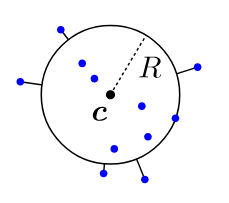
\includegraphics[width=4cm]{svdd}
	\end{center}
\end{wrapfigure}
From the dual we can get:
\begin{itemize}
	\item \textbf{Center}, a weighted average of points, with the \textit{stationary condition}
	\begin{equation}
		\mathbf{c} = \sum_{i=1}^{N} \alpha_i \mathbf{x}_i
	\end{equation}
	\item \textbf{Radius}, with the \textit{complementary slack}:
	\begin{align*}
		& \alpha_i \cdot (\lvert\lvert \mathbf{x}_i - \mathbf{c} \rvert\rvert^2 - S - \varepsilon_i) = 0\\
		& (C - \alpha_i) \cdot (-\varepsilon_i) = 0
	\end{align*}
	which yields for any point $i$ satisfying $0 < \alpha_i < C$ the equation $S=\lvert\lvert \mathbf{c} - \mathbf{x}_i \rvert\rvert^2$, or rather
	\begin{equation}
		R = \lvert\lvert \mathbf{c} - \mathbf{x}_i \rvert\rvert
	\end{equation}
\end{itemize}

\begin{observation}
	We can infer that any point inside the hyper sphere must have $\alpha_i = 0$, therefore the hyper sphere is only determined by points at the border of the distribution.
\end{observation}

\subsubsection{Comparison}
Compared to the Mahalanobis Distance, the SVDD model is more robust to the \textbf{skew} data, due to its ability to focus mainly on the border of the distribution. At the same time, for the same reason, it's more \textbf{"blurry"}

\subsubsection{Improvement}
The decision boundary of SVDD is greatly distorted by strong \textbf{outliers}, which may be interesting points or artifacts that we want to ignore. \\
To prevent this we need to robustify the model in two steps:
\begin{enumerate}
	\item Rewrite SVDD as the \textbf{constraint-free} optimization problem
	\begin{equation}
		\min_{S, \mathbf{c}, \mathbf{\varepsilon}} S + C \sum_{i=1}^N \underbrace{\max(0, \lvert\lvert \mathbf{x}_i - \mathbf{c}\rvert\rvert^2 - S)}_{\varepsilon(\mathbf{x}_i)}
	\end{equation}
	The added function $\max$ handles the two cases where the point is inside or outside of the hyper sphere. The problem is still convex and we can use gradient descent.
	\item Consider the alternative convex optimization problem
	\begin{equation}
		\min_{S, \mathbf{c}, \mathbf{\varepsilon}} S + C \sum_{i=1}^N \underbrace{\max(0, \lvert\lvert \mathbf{x}_i - \mathbf{c}\rvert\rvert - S)}_{\varepsilon^{(\text{new})}(\mathbf{x}_i)}
	\end{equation}
	Like the first step, the penalty $\varepsilon$ is triggered when the data point leaves the hyper sphere. However it grows \textbf{linearly} with the distance of the data point from the center. The problem is still convex and we can use gradient descent.
\end{enumerate}
% !TeX spellcheck = en_US
\newpage
\section{Clustering}
Clusters may carry important insights about the system or the process that generates the data such as the existence of different \textbf{states} (healthy or sick) or different \textbf{subprocesses}.

\begin{example}
	Methylation profiles of cancer cells organized into clusters, which often correlates with oncology categories. 
	
	\begin{center}
		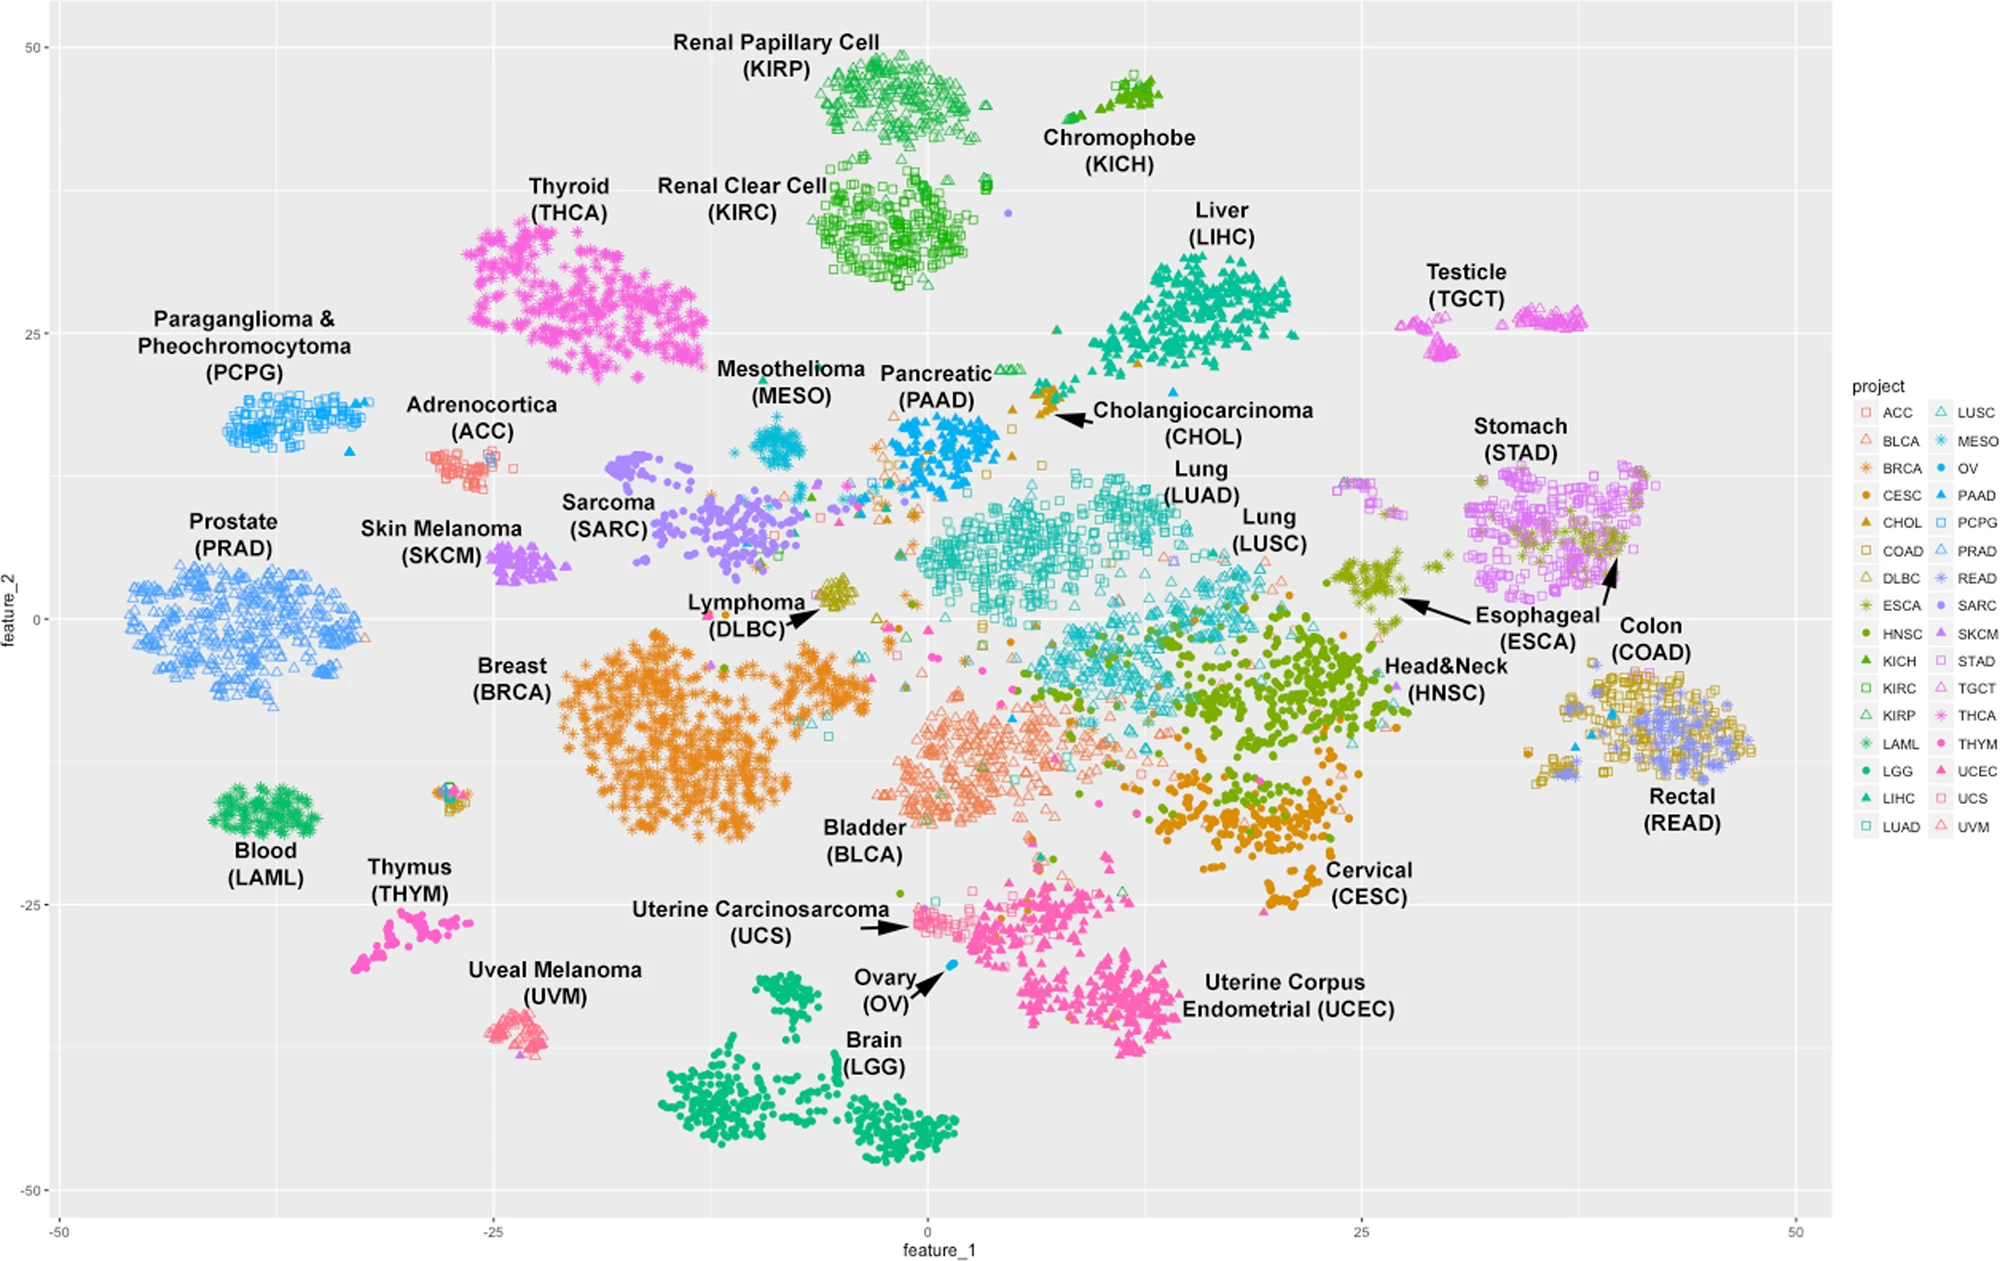
\includegraphics[scale=0.2]{clusters}
	\end{center}
\end{example}

\subsection{K-Means}
In the \textbf{centroid model} each cluster $k$ is represented by a \textbf{centroid} $\mu_k$ that lies in the same $d$-dimensional space as the data. It represents a prototype for points in that cluster, which are typically close to it.\\
The most well-known centroid-based technique is the \textbf{K-Means} algorithm, which works by iteratively updating the centroids and the assigned points until convergence.
\subsubsection{Algorithm}
Assuming a dataset $x_1, \ldots, x_N$, let $c_i \in \{1, \ldots, K\}$ be the cluster to which instance $i$ is assigned and let $C_k = \{i: c_i = k\}$ denote the set of instances in cluster $k$. Each cluster is represented by a centroid $\mu_k$ initialized at random. The algorithm is:
\begin{lstlisting}[mathescape=true]
	repeat
		$\forall_{i=1}^N: c_i = \arg\min_k \lvert\lvert \mathbf{x}_i - \mathbf{\mu}_k\rvert\rvert^2$
		$\forall_{i=1}^N: c_i = \mathbf{\mu}_k \leftarrow \frac{1}{\lvert C_k \rvert} \sum_{i \in C_k} \mathbf{x}_i$
	until convergence
\end{lstlisting}
\subsubsection{Optimization problem}
The algorithm can be interpreted as an attempt to \textbf{minimize}
\begin{equation}
	J(\mathbf{\mu}, \mathbf{c}) = \sum_{i=1}^N\lvert\lvert \mathbf{x}_i - \mathbf{\mu}_{c_i}\rvert\rvert^2 = \sum_{k=1}^K\sum_{i\in C_k}\lvert\lvert \mathbf{x}_i - \mathbf{\mu}_{k}\rvert\rvert^2
\end{equation}
which quantifies the amount of \textbf{dispersion} in each cluster.
\newpage
\noindent The \textbf{proof} for the two steps are:
\begin{enumerate}
	\item The objective is \textbf{sum-decomposable} with $c_1, c_2, \ldots, c_N$ and each cluster assignment can be optimized independently
	\begin{equation*}
		\arg\min_\mathbf{c} \sum_{i=1}^N \lvert\lvert \mathbf{x}_i - \mathbf{\mu}_{c_i}\rvert\rvert^2 = (\arg\min_{c_i}\lvert\lvert \mathbf{x}_i - \mathbf{\mu}_{c_i}\rvert\rvert^2)^N_{i=1}
	\end{equation*}
	\item Objective is also \textbf{sum-decomposable} with cluster prototypes and each of them can be optimized independently
	\begin{equation*}
		\arg\min_\mathbf{\mu}\sum_{k=1}^K\sum_{i\in C_k}\lvert\lvert \mathbf{x}_i - \mathbf{\mu}_{k}\rvert\rvert^2 = (\arg\min_{\mathbf{\mu}_k}\sum_{i\in C_k}\lvert\lvert \mathbf{x}_i - \mathbf{\mu}_{k}\rvert\rvert^2)^K_{k=1}
	\end{equation*}
\end{enumerate}

\begin{note}
	The clustering produced by the K-Means algorithm can be modeled by a \textbf{Voronoi diagram}.
	\begin{center}
		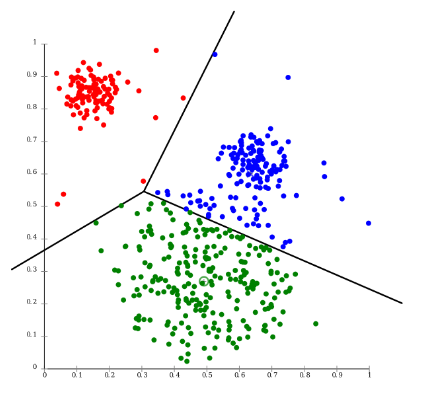
\includegraphics[scale=0.2]{voronoi}
	\end{center}
\end{note}

\subsubsection{Explained variance}
Data dispersion can be decomposed as follows:
\begin{align*}
	\frac{1}{N} \sum_{i=1}^{N} \lvert\lvert \mathbf{x}_i - \mathbf{\mu} \rvert\rvert^2 & = \frac{1}{N} \sum_k \sum_{i\in C_k} \lvert\lvert \mathbf{x}_i - \mathbf{\mu} \rvert\rvert^2\\
	& = \frac{1}{N} \sum_k \sum_{i\in C_k} \lvert\lvert \mathbf{x}_i - \mathbf{\mu}_k + \mathbf{\mu}_k - \mathbf{\mu} \rvert\rvert^2 \\
	& = \frac{1}{N} \sum_k \sum_{i\in C_k} [\lvert\lvert \mathbf{x}_i - \mathbf{\mu}_k\rvert\rvert^2 + \lvert\lvert \mathbf{\mu}_k - \mathbf{\mu} \rvert\rvert^2 +2(\mathbf{x}_i -\mathbf{\mu}_k)^T(\mathbf{\mu}_k - \mathbf{\mu})]\\
	& = \underbrace{\frac{1}{N} \sum_k \sum_{i\in C_k} \lvert\lvert \mathbf{x}_i - \mathbf{\mu}_k\rvert\rvert^2}_{\text{within-cluster dispersion}} + \underbrace{\frac{1}{N} \sum_k \sum_{i\in C_k} \lvert\lvert \mathbf{\mu}_k - \mathbf{\mu} \rvert\rvert^2}_{\text{between-cluster dispersion}} + \underbrace{\frac{2}{N} \sum_k \sum_{i\in C_k} +(\mathbf{x}_i -\mathbf{\mu}_k)^T(\mathbf{\mu}_k - \mathbf{\mu})}_{0}
\end{align*}
We define the \textbf{Calinski-Harabasz Index} as a criterion for evaluating the quality of a clustering solution. It's represented by the ratio of \textit{within-cluster dispersion} over \textit{between-cluster dispersion} multiplied by model simplicity:
\begin{equation}
	\text{Calinski-Harabasz}=\underbrace{\frac{\sum_k \sum_{i\in C_k} \lvert\lvert \mathbf{x}_i - \mathbf{\mu}_k\rvert\rvert^2}{\sum_k \sum_{i\in C_k} \lvert\lvert \mathbf{\mu}_k - \mathbf{\mu} \rvert\rvert^2}}_{\text{Model descriptive power}}\cdot \underbrace{\frac{N- K}{K-1}}_{\text{Model simplicity}}
\end{equation}
\paragraph{Choosing K} For a constant number of $K$ clusters, the algorithm optimizes the Calinski-Harabasz index. At the same time it helps on how to set that parameter. There are two approaches:
\begin{itemize}
	\item \textbf{Maximizing the index}: consider that the \textit{within-cluster dispersion} favors large $K$ while \textit{model simplicity} penalizes large $K$
	\item Looking for an \textbf{inflection} in the explained variance
	\begin{equation}
		\text{ExpVar}(\%) = \frac{\frac{1}{N} \sum_k \sum_{i\in C_k} \lvert\lvert \mathbf{\mu}_k - \mathbf{\mu} \rvert\rvert^2}{{\frac{1}{N}\sum_{i=1}^N \lvert\lvert \mathbf{x} - \mathbf{\mu}\rvert\rvert^2}}
	\end{equation}
\end{itemize}

\subsubsection{Limits}
K-Means has the following limits:
\begin{itemize}
	\item \textbf{Non convexity}: you initialize with values of the centroids that cover well the data. You repeat from $1$ to $100$ times and keep the solution that reaches the lowest objective
	\item \textbf{Low descriptive power}: even if the selected number of clusters is correct and the true optimum is reached, the solution may not be a desirable one, because the algorithm focuses on finding the clusters with least dispersion without paying attention to other aspects such as the margins between clusters
\end{itemize}

\subsection{Spectral clustering}
The dataset $\mathcal{D}$ is first converted into a \textbf{graph} $\mathcal{G}$ with an \textbf{adjacency matrix} $A$ indicating whether the distance between pair of points is below a certain threshold.\\
Then we need to find the \textbf{connected components} in the graph through an analysis of the adjacency matrix. To do that we:
\begin{enumerate}
	\item Represent $\mathcal{G}$ by the adjacency matrix $A$
	\item Build a derived matrix called \textbf{Laplacian}
	\begin{equation*}
		L = D-A
	\end{equation*}
	where $D=\text{diag}(A \cdot \mathbf{1})$ is the \textbf{degree matrix} and $\mathbf{1}$ is a vector of ones
	\item Perform \textbf{eigenvalue decomposition} of $L$, that is solving $L\mathbf{u} = \lambda \mathbf{u}$
	\item Eigenvectors $\mathbf{u}$ associated to eigenvalues $\lambda = 0$ are indicator vectors for the various connected components 
\end{enumerate}
\subsubsection{Formal derivation}
We can interpret the eigenvalues as the \textbf{variation of the eigenvector elements} between connected nodes. If $\lambda=0$, the eigenvector elements should be constant for each connected component.
\begin{align*}
	\lambda & = \mathbf{u}^TL\mathbf{u}\\
	& = \mathbf{u}^T(D-A)\mathbf{u}\\
	& = \sum_{i=1}^{N} \sum_{j=1}^{N} u_id_{ij}u_j - u_ia_{ij}u_j\\
	& = \qquad \vdots \\
	& = \frac{1}{2} \sum_{i=1}^{N} \sum_{j=1}^{N} a_{ij} (u_i - u_j)^2
\end{align*}

\begin{theorem}
	The number of zero eigenvalues of the Laplacian $L$, that is the multiplicity of the $0$ eigenvalue, equals the number of connected components $K$ of the graph.
\end{theorem}

The \textbf{last equation}, this \textbf{theorem} and the fact that \textbf{eigenvectors are orthogonal}, imply that the set of eigenvector with zero eigenvalue are indicator vectors for the connected components. Therefore, cluster membership is obtained by finding points that are embedded in the exact same location in eigenvector space.

\begin{center}
	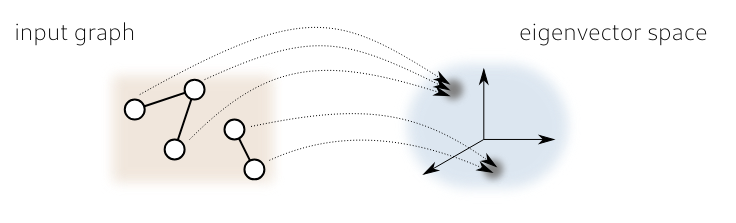
\includegraphics[scale=0.3]{clustin}
\end{center}

\subsubsection{Cheeger's Inequality}
\paragraph{Conductance}
Given the \textbf{conductance} of some set vertices $\mathcal{S}$ in the graph $\mathcal{G}$
\begin{equation}
	\phi(\mathcal{S}) = \frac{\text{edges}(\mathcal{S}, \overline{\mathcal{S}})}{\sum_{v \in \mathcal{S}}\text{degree}(v)}
\end{equation}
the conductance of the whole graph is defined as the minimum one among the sets that have at most half the volume of the complete graph
\begin{equation}
	\phi(\mathcal{G}) = \min_{\mathcal{S}:\text{vol}(\mathcal{S}) \leq \frac{\text{vol}(\mathcal{V})}{2}}\phi(\mathcal{S})
\end{equation}

\begin{definition}[Cheeger's Inequality]
	Let $\phi(\mathcal{G})$ denote the conductance of the graph $\mathcal{G}$. Then that can be related to the Laplacian's second eigenvalue as
	\begin{equation}
		\frac{\lambda2}{2} \leq \phi(\mathcal{G}) \leq \sqrt{2 \lambda_2}
	\end{equation}
\end{definition}

This inequality \textbf{implies} that if the conductance is low (natural 2-clustering), then the second eigenvalue $\lambda_2$ is low. Furthermore we can deduce that a low $\lambda_2$ will correspond to to low variations of the corresponding eigenvectors along connected nodes, hence it's predictive of cluster membership.

\subsubsection{Practice}
In practice spectral clustering can capture general cluster structures, including the ones that are non linearly separable. The quality of the clusters can substantially decrease if the data is noisy, but this is addressable through:
\begin{itemize}
	\item \textbf{Adjacency matrix}: try different parameters and ways of building it
	\begin{itemize}
		\item \textbf{Distance cutout}
		\begin{equation*}
			a_{ij}=I(\lvert\lvert \mathbf{x}_i - \mathbf{x}_j\rvert\rvert < \delta)
		\end{equation*}
		\item \textbf{Nearest neighbor}
		\item \textbf{Radial basis function}
		\begin{equation*}
			a_{ij} = \exp(- \frac{\lvert\lvert \mathbf{x}_i -\mathbf{x}_j \rvert\rvert}{2 \sigma^2} )
		\end{equation*}
	\end{itemize}
	\item \textbf{Laplacian matrix}: a variant of the standard one is the \textbf{normalized} one
	\begin{equation*}
		\tilde{L} = D^{-\frac{1}{2}}LD^{-\frac{1}{2}}
	\end{equation*}
	It gives more importance to regions of low connectivity.
	\item \textbf{Number of eigenvectors}: look for gaps in the eigenvalue spectrum, they usually indicate the separation between eigenvectors that code for cluster membership and those that code for variation within the cluster
\end{itemize}

\subsubsection{Conclusion}
The spectral clustering better focuses on the border. It can be useful as preparation step before K-Means. But it has several parameters to tune and clusters do not come with a prototype, making them hard to understand.
\end{document}
